\documentclass[]{article}
\usepackage[portuguese]{babel}
\usepackage{graphicx}
\usepackage[]{amsmath}

\title{Relatório de Circuito Digital}
\author{Erickson Müller, mat: 20230001178\\ Nicole Moritz, mat: 2221101074}
\date{03 de abril de 2024}

\begin{document}
\maketitle
\pagebreak
\section{Introdução}
	Nesta atividade será montado um circuito elétrico em protoboard utilizando o circuito digital apresentado pelo professor. Também serão identificadas a equação e tabela verdade do circuito.
	
	Os equipamentos utilizados na montagem deste circuito foram: Protoboard, Fonte, 1 switch DIP, 1 inverter, 2 LEDS, 2 resistores (74HC32 & 74HC04) e cabos elétricos.
	
	Para melhor entendimento do projeto, foi feito um circuito virtual na plataforma Tinkercad. Com o objetivo de economizar equipamentos e manter uma melhor organização no circuito físico, o qual tentou-se montar o mais fiel possível ao protótipo virtual.
	
\section{Circuito Digital}
	\includegraphics[scale=0.5]{images/circuito digital.png}
\section{Equação}
	\begin{equation}
		LED1 = \overline{(A.B)} + \overline{C} \label{eq:LED1.eq}
	\end{equation}
	
	\begin{equation}
		LED2 = \overline{C} \label{eq:LED2.eq}
	\end{equation}
	
\section{Tabela Verdade}
	\begin{tabular}{|c|c|c|c|}
		\hline
		\textbf{ A } & \textbf{ B } & \textbf{ C } & \textbf{LED1}\\
		\hline
		0 & 0 & 0 & 1 \\
		\hline
		0 & 0 & 1 & 1 \\
		\hline
		0 & 1 & 0 & 1 \\
		\hline
		0 & 1 & 1 & 1 \\
		\hline
		1 & 0 & 0 & 1 \\
		\hline
		1 & 0 & 1 & 1 \\
		\hline
		1 & 1 & 0 & 1 \\
		\hline
		1 & 1 & 1 & 0 \\
		\hline
	
	\end{tabular}
	\hfill
	\begin{tabular}{|c|c|c|c|}
		\hline
		\textbf{ A } & \textbf{ B } & \textbf{ C } & \textbf{LED2}\\
		\hline
		0 & 0 & 0 & 1 \\
		\hline
		0 & 0 & 1 & 0 \\
		\hline
		0 & 1 & 0 & 1 \\
		\hline
		0 & 1 & 1 & 0 \\
		\hline
		1 & 0 & 0 & 1 \\
		\hline
		1 & 0 & 1 & 0\\
		\hline
		1 & 1 & 0 & 1 \\
		\hline
		1 & 1 & 1 & 0 \\
		\hline
		
	\end{tabular}
	\\ \\
	Tabela Verdade do LED 1 
	\hfill
	Tabela Verdade do LED 2
	\\ 
	\\
	Pode-se perceber que o LED 1 vai ligar em todas as ocasiões, exceto quando as 3 entradas estiverem ativas. Já o LED 2 vai ligar sempre que a entrada C estiver desligada, não importando o valor das entradas A e B.
	\\
	\\
	Conforme analisado, a tabela verdade do circuito é a seguinte:
	\\
	\\
		\begin{tabular}{|c c c | c c |}
		\hline
		\textbf{} & \textbf{Entradas} & \textbf{} & \textbf{} &\hspace{-14mm}\textbf{Saídas}\\
		\hline
		\begin{tabular}{|c|c|c|c|c|}
		\hline
		\end{tabular}
		\textbf{ A } & \textbf{ B } & \textbf{ C } & \textbf{LED 1} & \textbf{LED 2}\\
		\hline
		0 & 0 & 0 & 1 & 1 \\
		\hline
		0 & 0 & 1 & 1 & 0 \\
		\hline
		0 & 1 & 0 & 1 & 1 \\
		\hline
		0 & 1 & 1 & 1 & 0 \\
		\hline
		1 & 0 & 0 & 1 & 1 \\
		\hline
		1 & 0 & 1 & 1 & 0\\
		\hline
		1 & 1 & 0 & 1 & 1 \\
		\hline
		1 & 1 & 1 & 0 & 0 \\
		\hline
		
	\end{tabular}
	
\section{Projeto do Circuito no Tinkercad}
	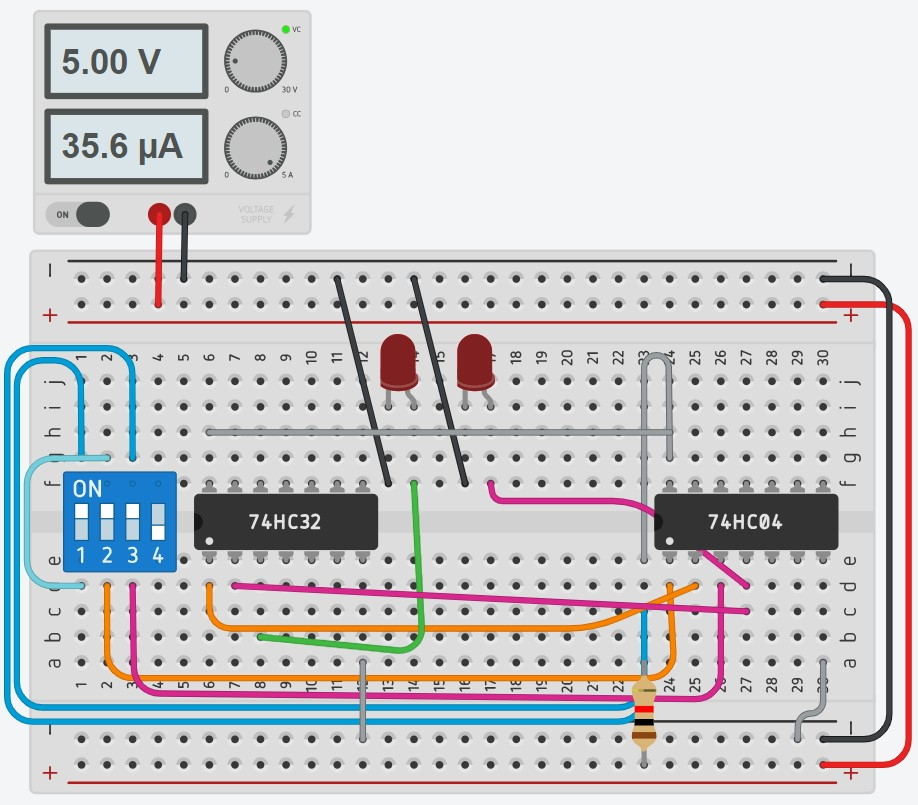
\includegraphics[scale=0.55]{images/tinkercad.jpg}
	\\
	Protótipo conforme representado na seção 1. Os 3 inputs ativos acabam retornando os 2 outputs inativos.\\ O Led 1 está à esquerda e o LED 2 está à direita. Este vai ligar sempre que 3 estiver no OFF, aquele vai apagar somente se todos os inputs estiverem no ON.
	
\section{Fotos do Circuito}


\section{Conclusão}
	Com a execução deste projeto aprendemos de forma prática como funciona a montagem de um circuito digital e quais são os usos de seus componentes. O circuito pode ser representado em três formas: graficamente (através do circuito lógico), com uma equação e com a tabela verdade. Montando esse circuito numa protoboard facilita a compreensão e visualização dessas três formas, ajudando a relacioná-las por inteiro.
	
	
\end{document}